\section{Component classes}

\subsection{StratifiedBuffer class}
An important component of the installation in the house model is a thermal buffer vessel. The vessel is a storage for hot water which serves as a reservoir for thermal energy. When large enough, the vessel can mediate the heat demand of the house by allowing fast discharge and slow charge rates. Slow charge rates enable the use of heat pumps and electric heating with modest power ratings. The buffer vessel therefore plays a key role in replacing gas boilers, without the involvement of high-power flow-through heaters. 

In modelling a thermal buffer vessel, it is customary to discretize the vertical temperature gradient by imposing a \emph{stratified} geometry. In this way, a stable configuration is achieved, with warmer (water) layers on top of colder layers in the vessel. Thus, convection phenomena can be neglected, and interlayer thermal transport occurs by diffusion, driven by the thermal downward gradient.

\begin{figure}[H]
	\centering
	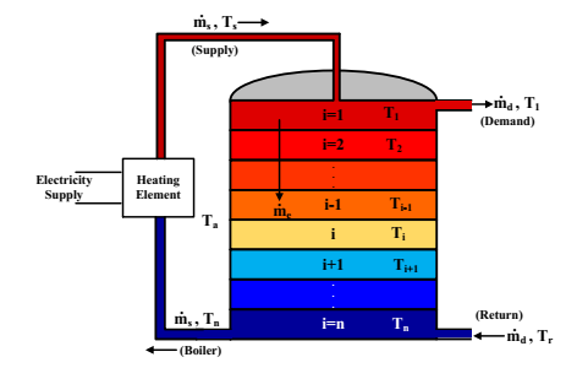
\includegraphics[width=0.5\columnwidth]{Pictures/stratified.png}
	\caption[Short title]{One-dimensional heat conduction in a stratified buffer vessel}
	\label{fig:stratified}
\end{figure} 

In the \textsf{housemodel/sourcesink} subpackage, a subpackage \textsf{buffervessels} is defined. The module buffer\_vessel.py contains a general class \textsf{StratifiedBuffer} with attributes and methods:

\lstinputlisting[label=lst:buffervessel, linerange={10-32}, 
caption={StratifiedBuffer class constructor}] 
{C:/Data/PROJECTS_NOVA/MCSE@BTO/FUTUREFACTORY/twozone_housemodel-git/housemodel/sourcesink/buffervessels/buffer_vessel.py}

The \textsf{StratifiedBuffer} object has the following attributes:

\begin{itemize}
	\item \textsf{n\_layers, hot\_node, cold\_node}. These parameters define the number of nodes occupied in the thermal network topology by the (layers of the) buffer vessel, as well as the connections (edges) to the other components of the network graph. In general, the hot top layer (node) of the vessel connects to the feed tube of a radiator or floor heating loop, The return line is then connected to the cold bottom layer (node) of the vessel. Additional connections to a heat pump, thermal collector or gas boiler can also be implemented.
	\item \textsf{volume, height, radius}. Geometrical parameters defining the size of the (cylindrical) buffer vessel.
	\item \textsf{temperatures}. An array of dimension \textsf{n\_layers} containing the temperatures of all layers of the buffer vessel.
\end{itemize}

Furthermore, the \textsf{StratifiedBuffer} object has a number of methods including:

\begin{itemize}
	\item \textsf{setters and getters}. These methods set or alter the geometrical attributes of the buffer vessel.
	\item \textsf{model functions}. These methods describe the change in temperature of the layers of the buffer vessel. The return values may serve as derivatives for an ODE solver.
\end{itemize}

\lstinputlisting[label=lst:buffervessel, linerange={47-97}, 
caption={StratifiedBuffer model function}] 
{C:/Data/PROJECTS_NOVA/MCSE@BTO/FUTUREFACTORY/twozone_housemodel-git/housemodel/sourcesink/buffervessels/buffer_vessel.py}























\newpage